% !TeX root = ../../thesis.tex

With the method described in the algorithm \ref{alg:simil_1}, we created a figure where the metrics are presented with increasingly different datasets: Figure \ref{fig:lineplot}.
%Then we compared the difference in the metric across iterations, rendering figure \ref{fig:boxplot}.

%TC:ignore
\begin{figure}[htbp]
\centering
\caption[Plot showing the variation of different metrics over increasingly changed datasets.]{Plot showing the decrease of the metric over increasingly changed datasets. The X axis represents the number of columns mutated. The Y axis represents the value of the metric and the hue represents the algorithm used to calculate the metric.}\label{fig:lineplot} 
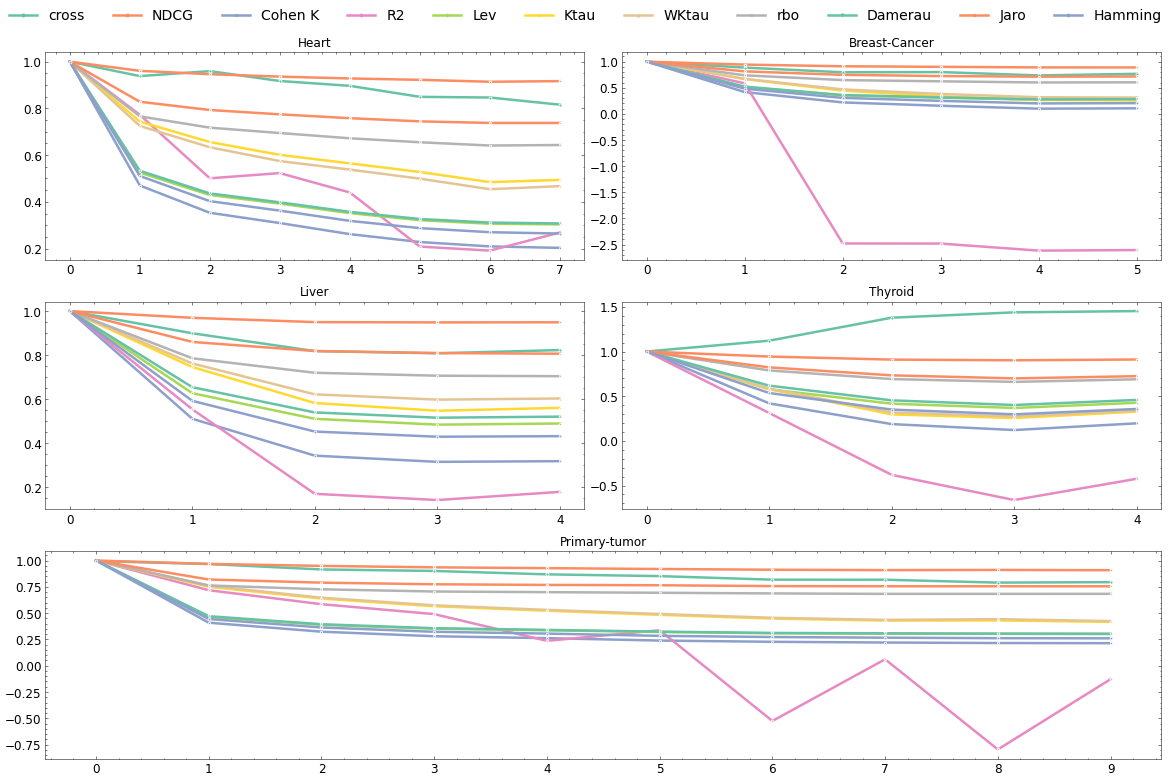
\includegraphics[scale=0.37]{figures/multiple_datasets.png}
\end{figure}
%TC:endignore

The number of repetitions and how that impacts the variance of the scores is shown in Figure~\ref{fig:facet_plot}.


%TC:ignore
\begin{figure}[htbp]
    \centering
    \caption{Heatmap showing the variance of different repetitions for every metric and the number of different columns changed. X is the metric. Y is the number of repetitions and the number of columns. This was obtained by getting the variance of all values from all datasets.  }\label{fig:facet_plot} 
    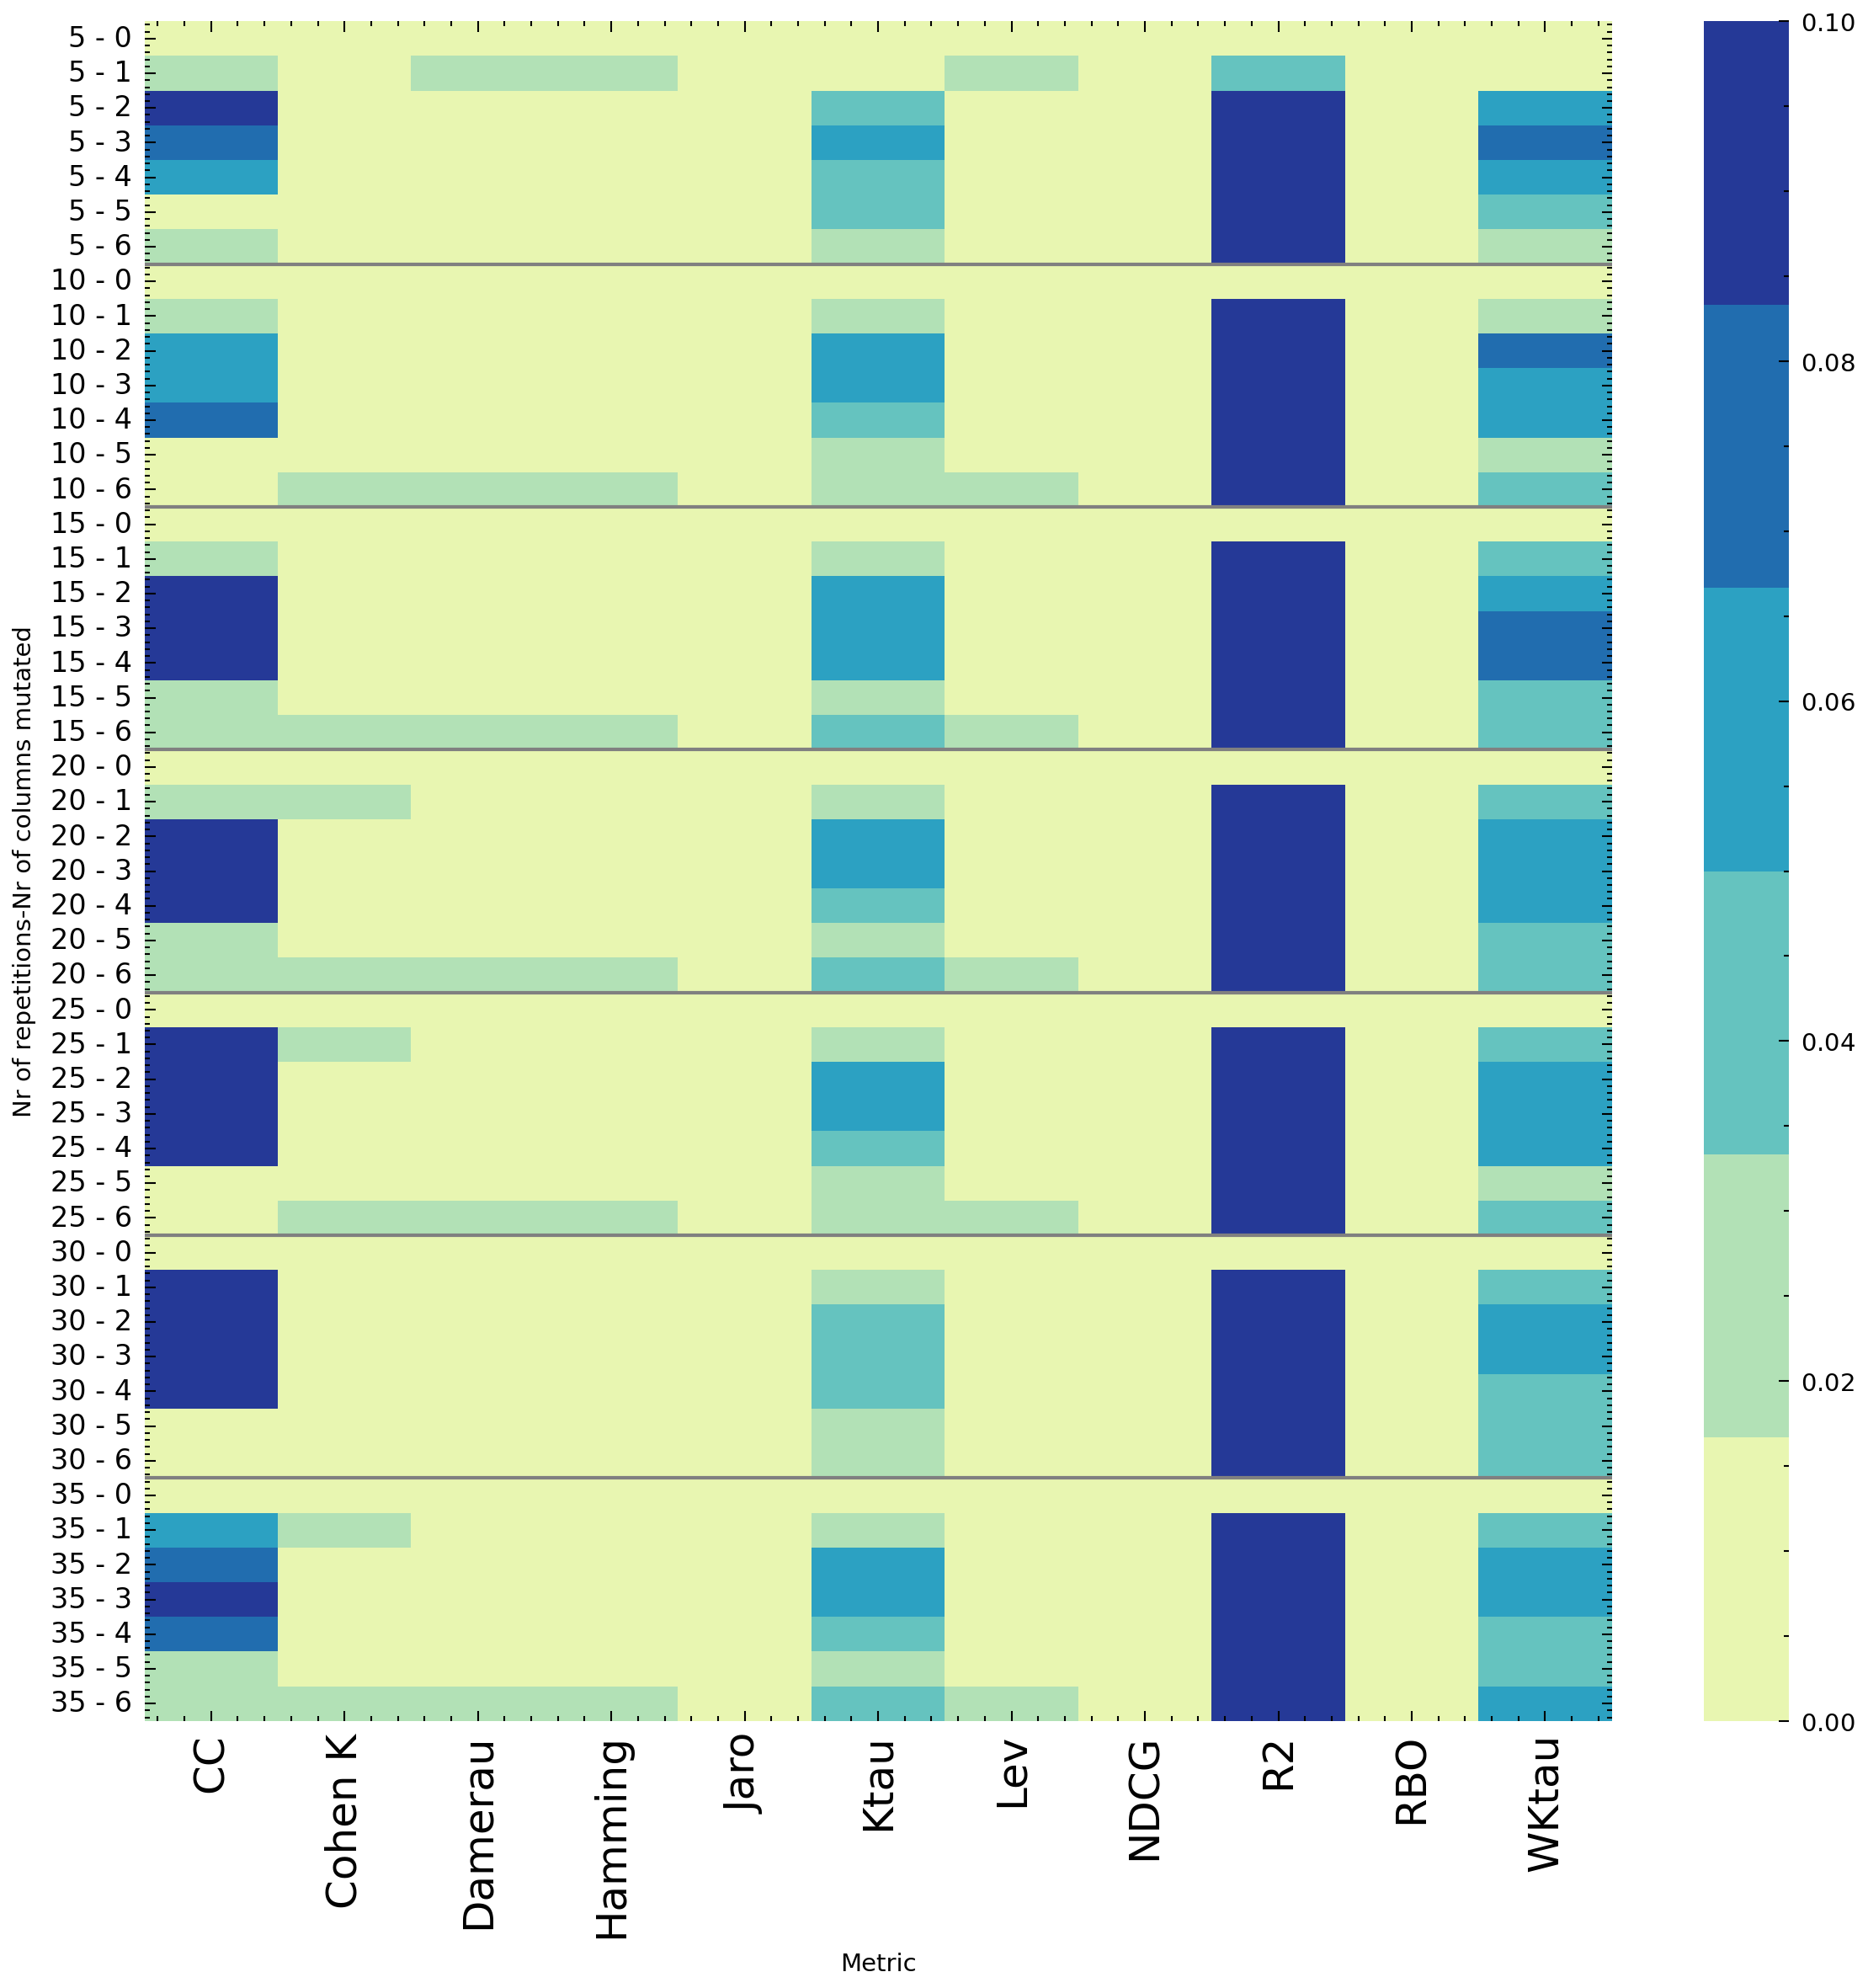
\includegraphics[scale=0.60]{figures/heatmap-runs.png}
    \end{figure}
    %TC:endignore

As for the test for the synthetic and real dataset, the results are displayed in figure~\ref{fig:synth_result} and ~\ref{fig:synth_heat}. This is the metrics distribution for the comparison of the 5 mentioned datasets and the synthetic counterpart generated as stated in the methods section.
    %TC:ignore
\begin{figure}[htbp]
    \centering
    \caption{Distributions of the metrics results comparing 5 synthetic and real datasets across 3 different generation methods}\label{fig:synth_result} 
    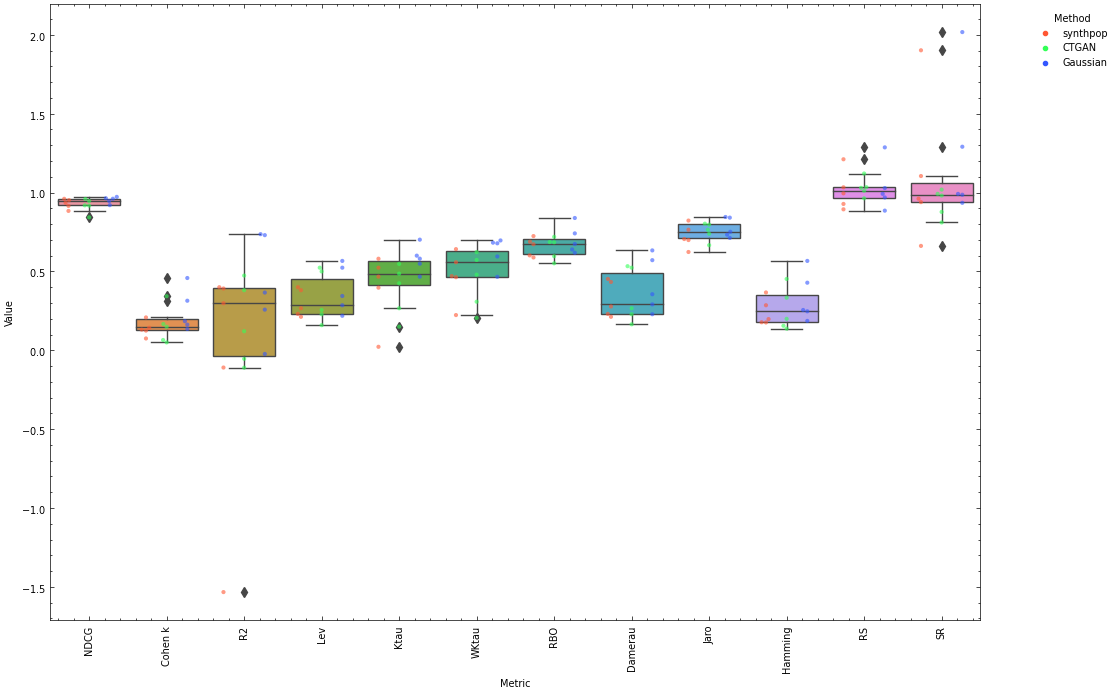
\includegraphics[scale=0.60]{figures/synthetic_violin_swarm_colored_by_group_custom.png}
    \end{figure}
    
    \begin{figure}[htbp]
        \centering
        \caption{Values and comparison of the metrics results comparing 5 synthetic and real datasets across 3 different generation methods}\label{fig:synth_heat} 
        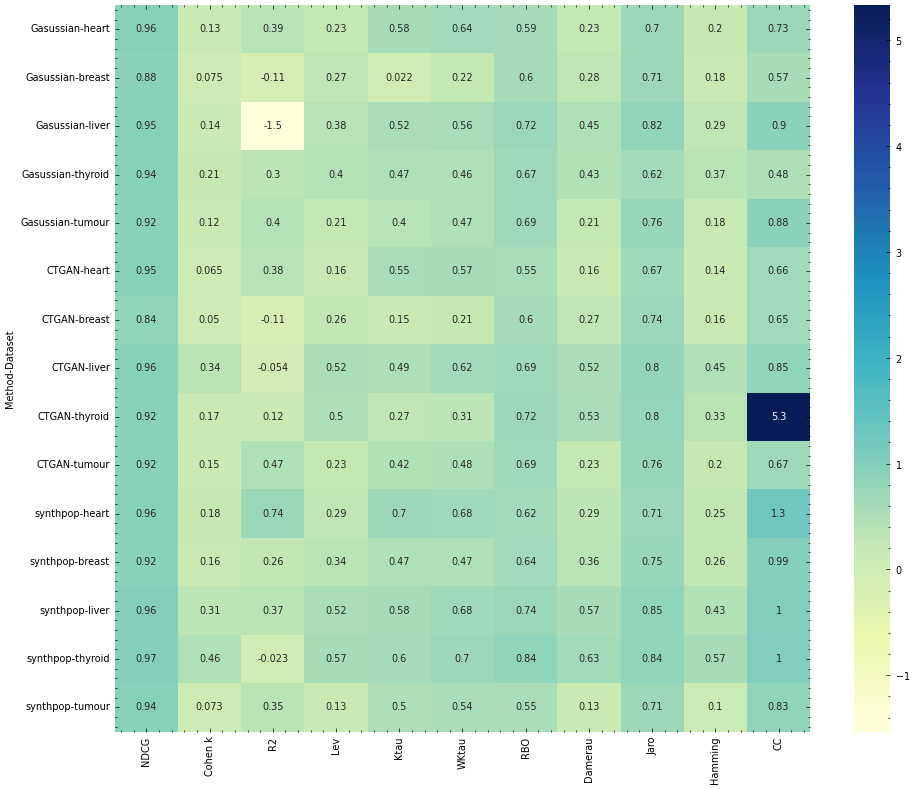
\includegraphics[scale=0.60]{figures/heatmap-synth.png}
        \end{figure}
    %TC:endignore